\documentclass[12pt]{article}
\usepackage{fullpage,url,amssymb,epsfig,color,xspace,tikz,amsmath}
\usepackage{graphicx}
\usepackage{float}
\usepackage[pdftitle={CS 486 Assignment 1},
pdfsubject={University of Waterloo, CS 486, Winter 2024},
pdfauthor={Arne Storjohann}]{hyperref}
\usepackage{algpseudocode,enumitem,calc,multicol}

\usepackage{listings}
\lstset{%
        language=C++,
        keepspaces=true,
        basicstyle=\small\ttfamily,
       commentstyle=\footnotesize\itshape{},
       identifierstyle=\slshape{},
       keywordstyle=\bfseries,
       numbers=left,
       numberstyle=\tiny{},
       numberblanklines=false,
       inputencoding={utf8},
       columns=fullflexible,
       basewidth=.5em,
        fontadjust=true,
        tabsize=3,
        emptylines=*1,
       breaklines,
       breakindent=30pt,
        prebreak=\smash{\raisebox{-.5ex}{\hbox{\tiny$\hookleftarrow$}}},
    escapeinside={//*}{\^^M} % Allow to set labels and the like in comments starting with //*
	}


\renewcommand{\thesubsection}{Problem \arabic{subsection}}

\begin{document}

\begin{center}
  {\Large\bf University of Waterloo}\\ \vspace{3mm}
  {\Large\bf CS 486, Winter 2024}\\ \vspace{2mm}
  {\Large\bf Assignment 4}\\ \vspace{3mm}
\end{center}

\definecolor{care}{rgb}{0,0,0}
\def\question#1{\item[\bf #1.]}
\def\part#1{\item[\bf #1)]}
\newcommand{\pc}[1]{\mbox{\textbf{#1}}} % pseudocode

%%%%%%%%%%%%%%%%%%%%%%%%%%%%%%%%%%%%%%%%%%%%%
\subsection{} 
\begin{enumerate}

\part{a} 
The Bayesian network is:
\begin{figure*}[h]
	\center
	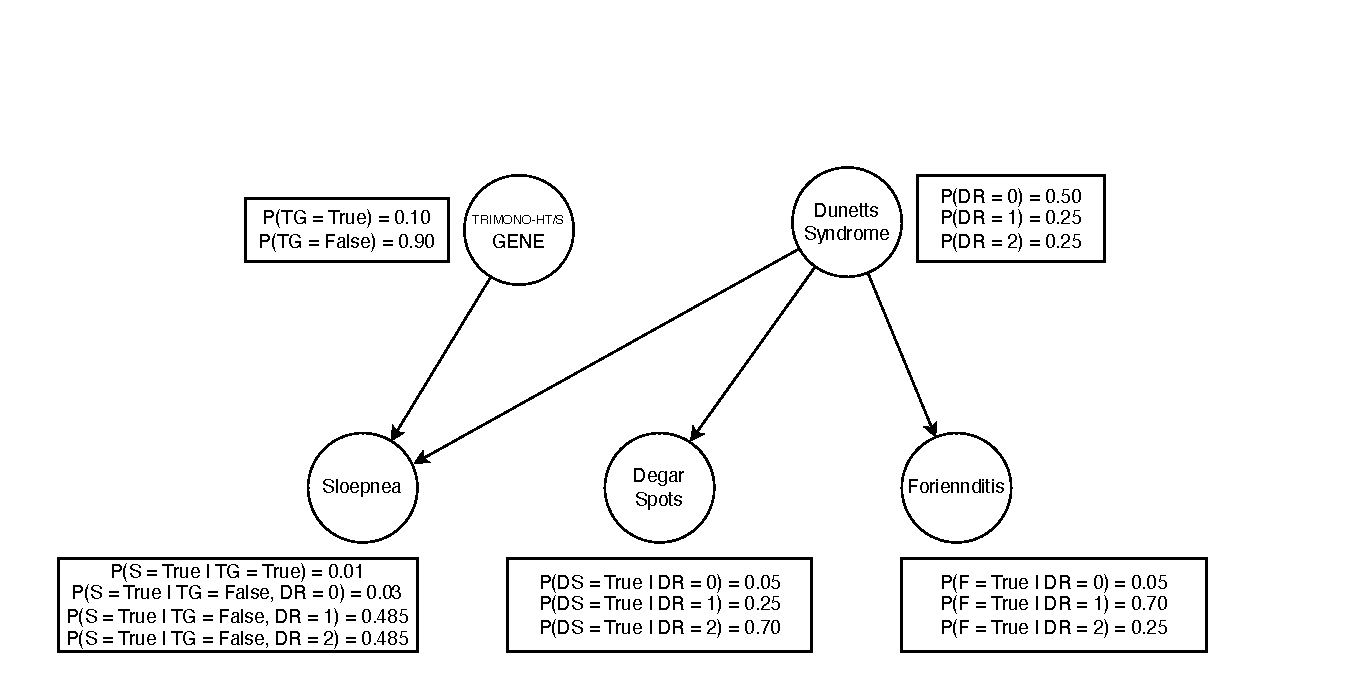
\includegraphics[width=\linewidth]{Q1a.pdf}
\end{figure*}

\part{b} 

\part{c} 

\end{enumerate}


%%%%%%%%%%%%%%%%%%%%%%%%%%%%%%%%%%%%%%%%%%%%%
%%%%%%%%%%%%%%%%%%%%%%%%%%%%%%%%%%%%%%%%%%%%%
\newpage
\subsection{} 
\begin{enumerate}
\part{a} 

\part{b} 

\part{c} 

\end{enumerate}

%%%%%%%%%%%%%%%%%%%%%%%%%%%%%%%%%%%%%%%%%%%%%
%%%%%%%%%%%%%%%%%%%%%%%%%%%%%%%%%%%%%%%%%%%%%

\end{document}
